%! Author = joeda
%! Date = 2022-12-19

% Preamble
\documentclass[11pt]{article}
\linespread{2}
\usepackage{geometry}
\geometry{margin=1in}
% Packages
\usepackage{amsmath}
\usepackage{graphicx}
\usepackage{caption}
\usepackage{subcaption}
\usepackage{subfigure}
\usepackage{biblatex}
%\usepackage[backend=biber]{biblatex}

\usepackage{blindtext}%section management
\usepackage{xcolor} %color management

\newcommand\myworries[1]{\textcolor{red}{#1}}

\usepackage[utf8]{inputenc} % Pour les accents
\usepackage[english]{babel}  % Language hyphenation and typographical rules
\usepackage{csquotes}
\usepackage{hyperref}
\usepackage{amsfonts}


\usepackage{booktabs}


\addbibresource[backend=biber]{reference.bib}
% Document
\begin{document}

\section{Data Analysis}

    The first step of any ML project is to analyse the data available to us. We will already split our data between
    training and validation just to simplify our analysis here.

    First, our private data from CIUSSS. We will first look at the distribution of the classes. As we can see in
\ref{fig:hist_ciusss}, the classes are not balanced. We will need to take this into account when training our model.


While we tried to provide a minimum of examples for each class in the validation dataset, we still observe a class imbalance.
We will therefore need to be careful not only to rely on a basic loss for things like a hyperparameter search if we want to
have the best model in more than the over-represented categories. We could, for example, ponder the loss with different weights
by classes



\begin{figure}[h]
     \centering
     \begin{subfigure}[b]{0.45\linewidth}
         \centering
         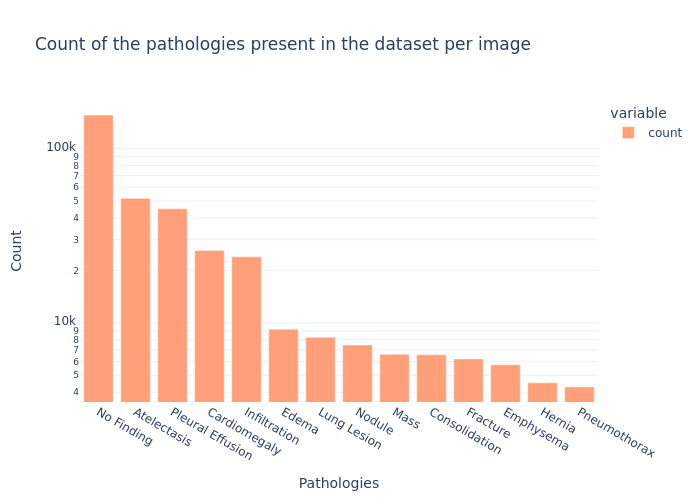
\includegraphics[width=\linewidth]{plots/histogram_ciusss_train}
         \caption{ChexPert's training dataset}
         \vspace{4ex}
         \label{fig:histogram_ciusss_train}
     \end{subfigure}
     \hfill
     \begin{subfigure}[b]{0.45\linewidth}
         \centering
         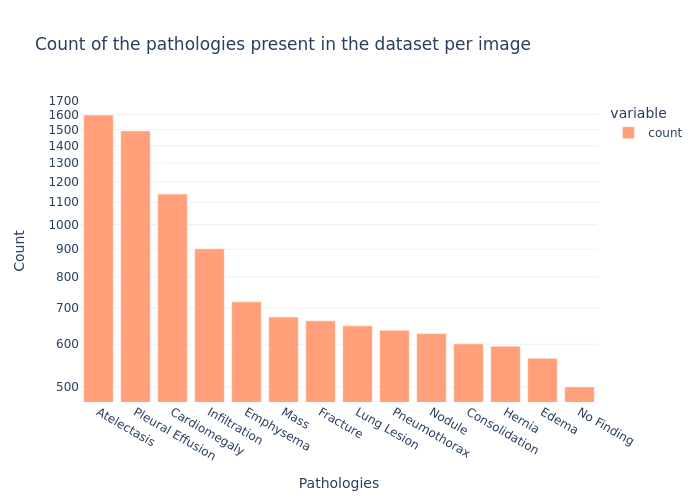
\includegraphics[width=\linewidth]{plots/histogram_ciusss_valid}
         \caption{ChexPert's validation dataset}
         \vspace{4ex}
         \label{fig:histogram_ciusss_valid}
     \end{subfigure}


     \begin{subfigure}[b]{0.45\linewidth}
         \centering
         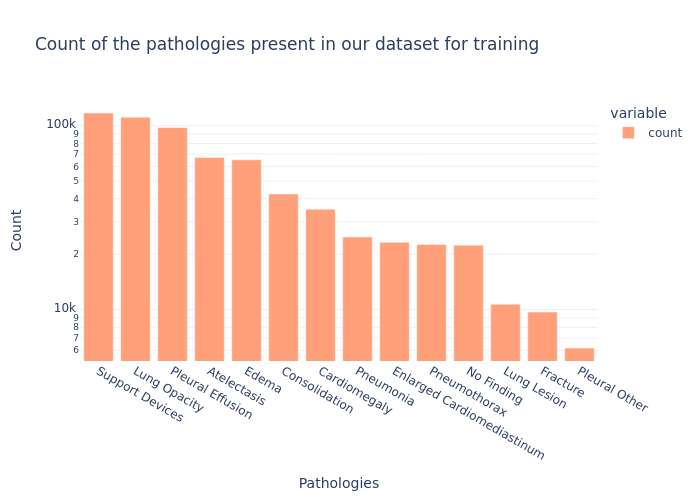
\includegraphics[width=\linewidth]{plots/histogram_chexpert_train}
         \caption{CIUSSS's training dataset}
         \vspace{4ex}
         \label{fig:histogram_chexpert_train}
     \end{subfigure}
     \hfill
     \begin{subfigure}[b]{0.45\linewidth}
         \centering
         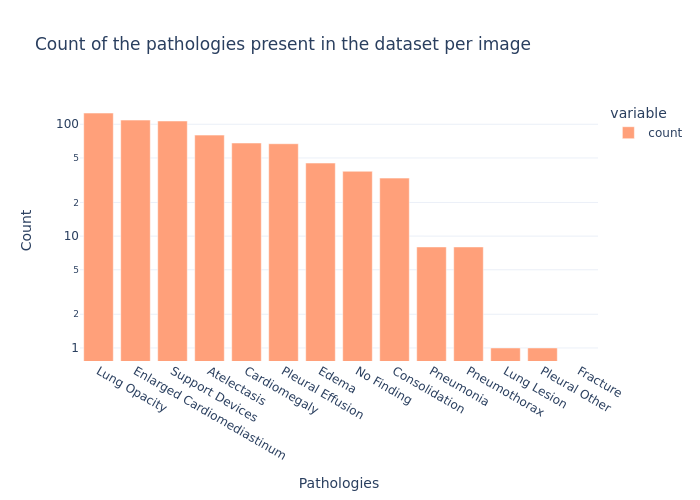
\includegraphics[width=\linewidth]{plots/histogram_chexpert_valid}
         \caption{CIUSSS's validation dataset}
         \vspace{4ex}
         \label{fig:histogram_chexpert_valid}
     \end{subfigure}

     \caption{Histogram for the different labels present in the CIUSSS and CheXpert dataset}

\end{figure}



    Another important thing to look at could be the correlation between diseases, to identify potential biases in the data.


\begin{figure}[!h]
     \centering
     \begin{subfigure}[b]{0.45\linewidth}
         \centering
         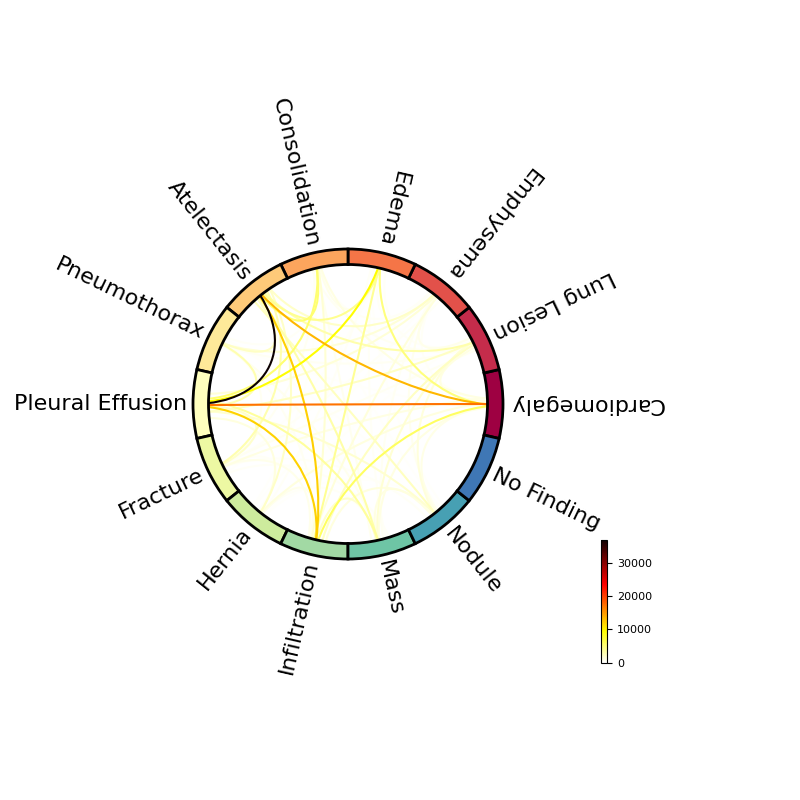
\includegraphics[width=\linewidth]{plots/chords_ciusss_train}
         \caption{CIUSSS's training dataset}
         \vspace{4ex}
         \label{fig:chords_ciusss_train}
     \end{subfigure}
     \hfill
     \begin{subfigure}[b]{0.45\linewidth}
         \centering
         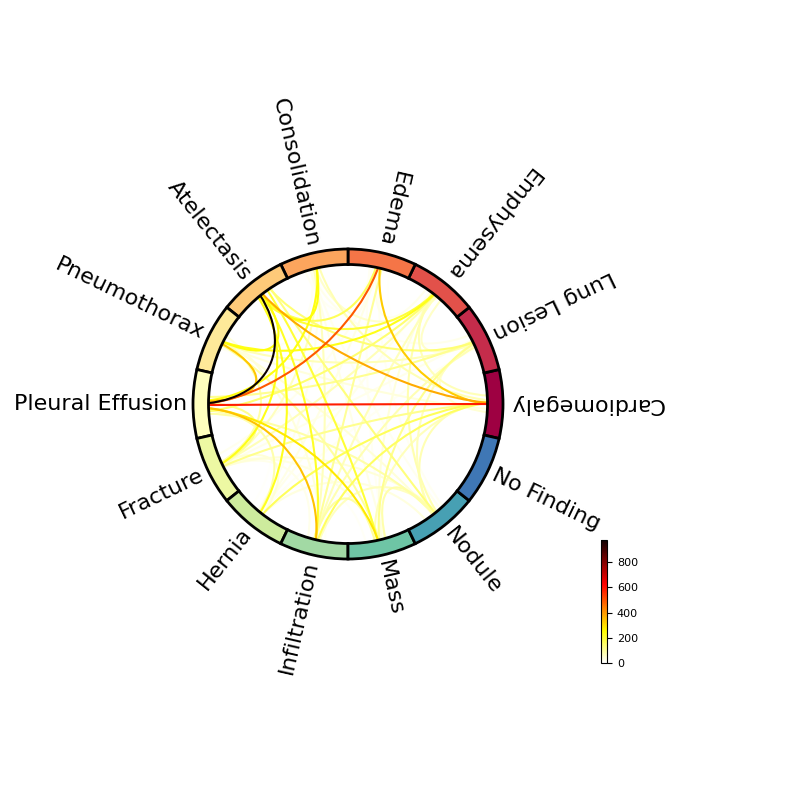
\includegraphics[width=\linewidth]{plots/chords_ciusss_valid}
         \caption{CIUSSS's validation dataset}
         \vspace{4ex}
         \label{fig:chords_ciusss_valid}
     \end{subfigure}


     \begin{subfigure}[b]{0.45\linewidth}
         \centering
         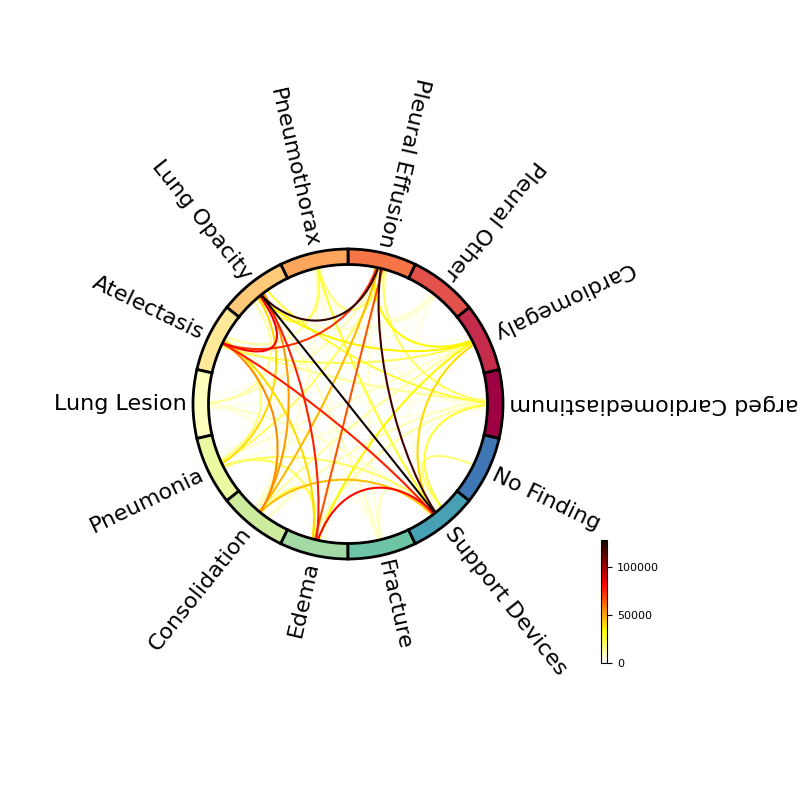
\includegraphics[width=\linewidth]{plots/chords_chexpert_train}
         \caption{CheXpert's training dataset}
         \vspace{4ex}
         \label{fig:chords_chexpert_train}
     \end{subfigure}
     \hfill
     \begin{subfigure}[b]{0.45\linewidth}
         \centering
         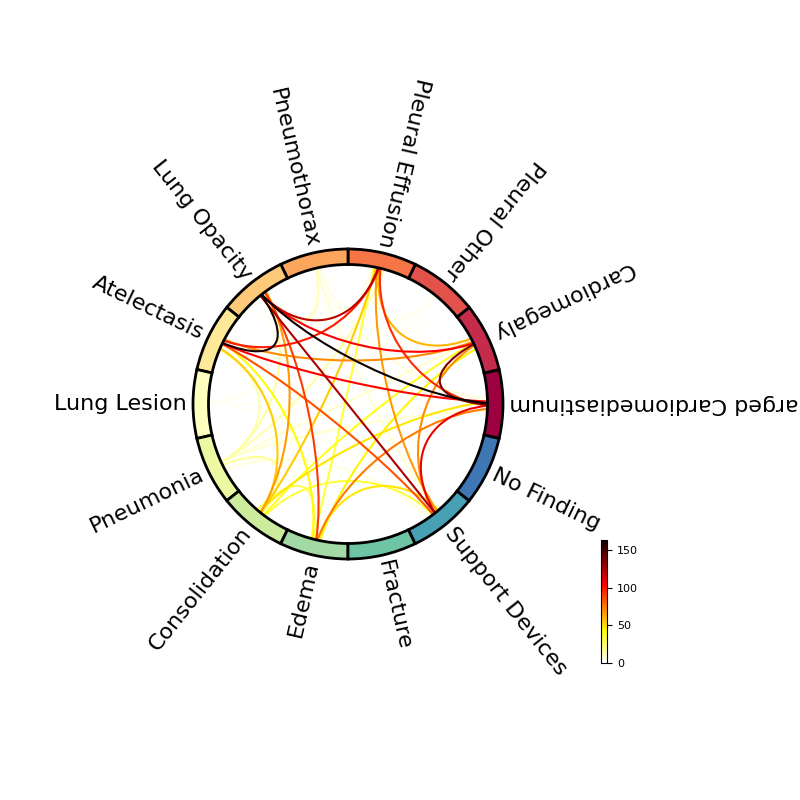
\includegraphics[width=\linewidth]{plots/chords_chexpert_valid}
         \caption{CheXpert's validation dataset}
         \vspace{4ex}
         \label{fig:chords_chexpert_valid}
     \end{subfigure}

     \caption{Histogram for the different labels present in the CIUSSS and CheXpert dataset}

\end{figure}


    Looking at the Chexpert's correlation graph (see \ref{fig:chords_chexpert_train} and \ref{fig:chords_chexpert_valid}), we can see that the correlation between diseases is quite high. This is slightly worrying, as it means that the data could be biased
    towards a specific disease. We can also see that the correlation is higher in the validation dataset than in the training
    dataset. This is expected, as the validation dataset is smaller and therefore more likely to have a higher correlation
    between diseases.

%    We can also look at the correlation between diseases and the age of the patient. We can see that the correlation is not
%    very high, which is good. This means that the data is not biased towards a specific age group. We can also see that the
%    correlation is higher in the validation dataset than in the training dataset. This is expected, as the validation dataset
%    is smaller and therefore more likely to have a higher correlation between diseases and age.

    However, when we look at the CIUSSS's correlation graph (see \ref{fig:chords_ciusss_train} and \ref{fig:chords_ciusss_valid}), we observe a way lower correlation level between pathologies.
    It might also be due to a difference in the population but this explanation does not seem quite likely

    Assuming the preponderance of diseases is the same between the population visiting the Stanford's hospital and
    the CIUSSS CCSMTL, we are left to assume that the quality of the data is different from the Stanford dataset. Whether it is better or worst is to verify.


    \section{Preparing the data}



    Before sending our data into an ML algorithm , we need to think about the preprocessing that we can apply on it to facilitate
    the learning process. For our use case, with deep learning models, it is typical to split this step in two part : augmentations
    and normalization.


    For data augmentations, we used a combination of random horizontal flipping of the image, as the lungs are symmetrical,color jittering, to add random noise
    in the images, affine transformation (see albumentation's documentation \footnote{https://albumentations.ai/docs/api_reference/augmentations/geometric/transforms/}), and a mix of griddistortion and Elastic transformation to simulate a greater
    variance in the shape of the specified pathologies. All the augmentations were done with Albumentations, as to avoid making mistakes
    by writing our own\cite{albumentations}.

    Data augmentation such as this serves two purposes. The first one is to allow the model to generalize better, as it is given
    a wider variety of examples (albeit partially synthetic examples) . The second purpose is to avoid overfitting as the model will
    have a harder time simply memorizing the examples instead of actually learning the desired characteristic within the image.

    The second step, normalization, serves to assure that the distribution of the image stay within a specified norm. It is typical
    to bring the images values between 0 and 1, and , if using a pretrained model as it is our case, to normalize the data
    according to the specified mean and standard deviation value of the images used to pretrain the model (in our case ImageNet).

    It is also possible to use histogram equalization. This method will normalize image with respect to local values instead of the global maximum and minimum.
    Improving on this idea we used the Contrast Limited Adaptive Histogram Equalization \footnote{see https://towardsdatascience.com/clahe-and-thresholding-in-python-3bf690303e40}
    to further improve the normalization of our images. We hope this will help with the cross-generalization of our model on the different datasets.

    %As can be seen here \ref{figure}, the usage of clahe vs only min-max normalization did result in a slight improvement


\begin{figure}[!h]
     \centering
     \begin{subfigure}[b]{0.45\linewidth}
         \centering
         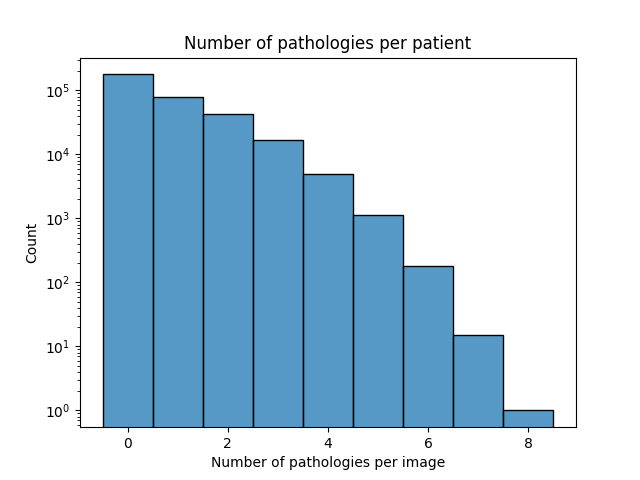
\includegraphics[width=\linewidth]{plots/disease_count_ciusss_train}
         \caption{CIUSSS's training dataset}
         \vspace{4ex}
         \label{fig:count_ciusss_train}
     \end{subfigure}
     \hfill
     \begin{subfigure}[b]{0.45\linewidth}
         \centering
         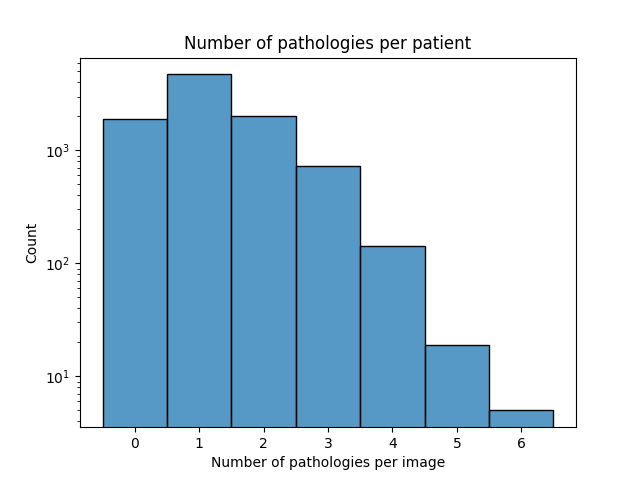
\includegraphics[width=\linewidth]{plots/disease_count_ciusss_valid}
         \caption{CIUSSS's validation dataset}
         \vspace{4ex}
         \label{fig:count_ciusss_valid}
     \end{subfigure}


     \begin{subfigure}[b]{0.45\linewidth}
         \centering
         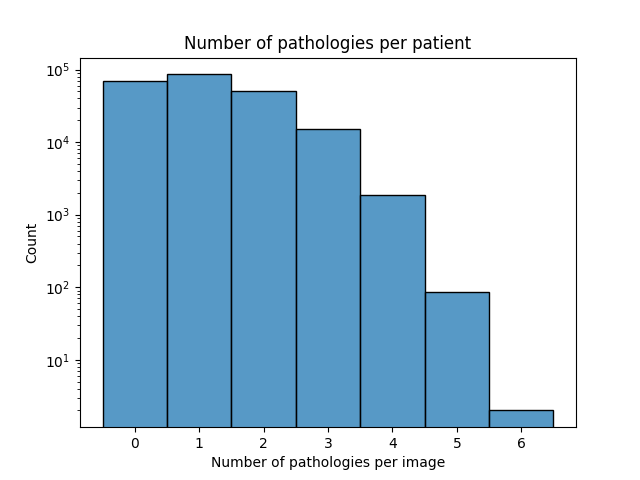
\includegraphics[width=\linewidth]{plots/disease_count_chexpert_train}
         \caption{CheXpert's training dataset}
         \vspace{4ex}
         \label{fig:count_chexpert_train}
     \end{subfigure}
     \hfill
     \begin{subfigure}[b]{0.45\linewidth}
         \centering
         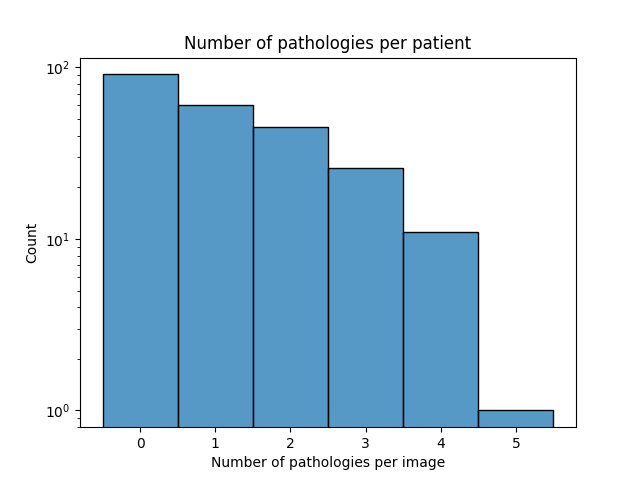
\includegraphics[width=\linewidth]{plots/disease_count_chexpert_valid}
         \caption{CheXpert's validation dataset}
         \vspace{4ex}
         \label{fig:count_chexpert_valid}
     \end{subfigure}

     \caption{Histogram for the different labels present in the CIUSSS and CheXpert dataset}

\end{figure}

    Now come the tricky part where we get in the wood inside of getting out. While the data processing described earlier
    is accurate, it is also general and do not reflect the specificty of our data! Two main problem arise.

    Firstly, as mentionned earlier, the data is unbalanced! While typically , we would simply undersample the over-represented
    categories or the opposite, oversample the under-represented classes, it is not an option here. Looking closely at the data \ref{fig:classes_per_image},
    we can see our problem is not a simple classification, but a multilabel classification tasks where more than one class might be present
    in the input! We also see that we have a lot of images with no pathology at all. This is a problem as it means that the model will be biased toward answering no pathology are present. We therefore need to undersample this category!



    To resolve this , we can try some version of undersampling to partially mitigate the imbalance, but a better solution exists. We can assign each positive example
    of a class with a weight, therefore increasing the importance of the positive examples of the under-represented classes. This is
    done by using the class weights parameter of the loss function. This is a good solution, but it is not perfect of course as one class might have a higher preponderance in the loss
    function.

    To mitigate this, we could use a weighted loss function, which will weight the loss of each class according to the class weights. This could be interesting as a future improvement.


    Secondly, our data does not come in the form of a simple image. The input is composed of multiple images present in the patient file for a specific exam, typically between 1 and 4 images. While a RNN could be use to deal
    with a sequence of image, no such model exist for medical imaging. Instead, we will use a CNN to process each image independently, and combine the output with a simple addition before applying the sigmoid activation function.

    To further simplify the model, we also explored two other option

    \subsection{Option 1 : Only use 1 frontal image}
        Our first attempt was to use only one frontal image per patient. This is a simple solution, but it is not optimal as it does not take into account the other images present in the patient file.
        However, we quickly realize that this was not a good idea as the model was underperforming with some specific pathologies. This was most
        likely due to these pathologies having been identified through the other images present in the patient file, and especially the lateral images.
        Further investigation confirmed our hypothesis, as some pathologies like pleural effusion were mostly confirmed by the lateral images.

    \subsection{Option 2 : Use two different set of weights for the feature extraction of frontal vs lateral images}

        To ensure the model learned in an optimal manner from both lateral and frontal images, we tried to use two different set of weights for the feature extraction of frontal vs lateral images. This however
        effectively double the number of parameters to train, and led to a significant increase in the model capacity and overfitting. This option was therefore also rejected.

        % link to document?
    Finally , we opted to use two of the images present in the patient file, and to combine the output of the CNN with a simple addition before applying the sigmoid activation function. This is a simple solution, but it is not optimal as it does not take into account the other images present in the patient file.
    It however will help simplify training as the model will almost always have the same number of input images (2, more rarely 1), and will also help with the generalization of the model as it will be trained on a wider variety of images.

    To undersample the empty images, we will ponder them with a weight of 0.1, and the other images with a weight of 1. This will effectively leave us with a dataset containing the equivalent of only about 20 000 empty images.





    \section{Model architecture}

    \subsection{Model 1 : DenseNet \cite{densenet}}


    \begin{figure}[h]

         \centering
         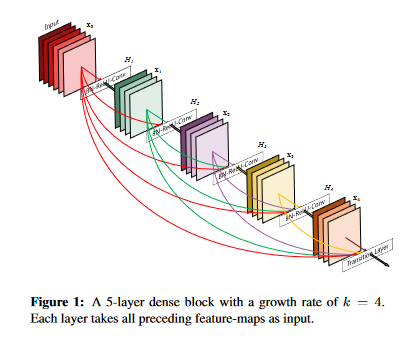
\includegraphics[width=0.8 \textwidth]{plots/densenet_figure}
         \caption{Figure 1 from the densenet paper \cite{densenet}. It shows how the layers are all interconnected}
         \label{fig:densenet_figure}

    \end{figure}

        The densenet model is a CNN model that is composed of dense blocks. Each dense block is composed of a series of convolutional layers,
        each of which is connected to all the previous layers in the block (see \ref{fig:densenet_figure}). This allows the model to learn features at different scales, and to
        combine them in a more efficient manner. The model is also composed of a transition layer, which is used to reduce the number of feature maps
        and to control the growth of the model. The model is also composed of a classifier, which is composed of a global average pooling layer and a fully connected layer.



        This model released in 2018 improved on ResNet with its dense blocks, and was the state of the art for a while. The stanford team working on ChexNet found it was the best model available to achieve the highest AUC on CXR images \cite{chexnet}.


    \subsection{Model 2 : ConvNeXt \cite{convnext}}


\begin{figure}[h]

     \centering
     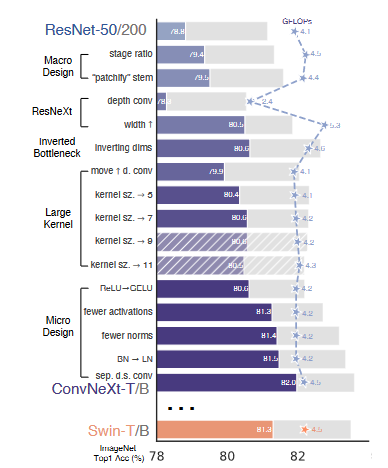
\includegraphics[width=0.8 \textwidth]{plots/convnext_graph}
     \caption{Figure 2 from the ConvNeXt paper \cite{convnext}. It details the different improvement made to the
     resnet architecture and the gain in performance obtained following each modification.}
     \label{fig:convnext}

\end{figure}

        The ConvNeXt model is another CNN model, this time released in 2020 and improving on the default Resnet architecture once again.
        They gradually implemented many of the features of vision transformers in order to "modernize" the typical CNN architecture. In doing sp,
        they created an architecture which outperformed many SOTA models on the ImageNet competititon.

        The details of these modifications can be seen in the figure \ref{fig:convnext}, which is taken from their paper.
        It replaced densenet as the "default" convolutionnal model


    \subsection{Model 3 : EfficientNet \cite{efficientnet} and YOLO \cite{yolo}}


\begin{figure}[h]

     \centering
     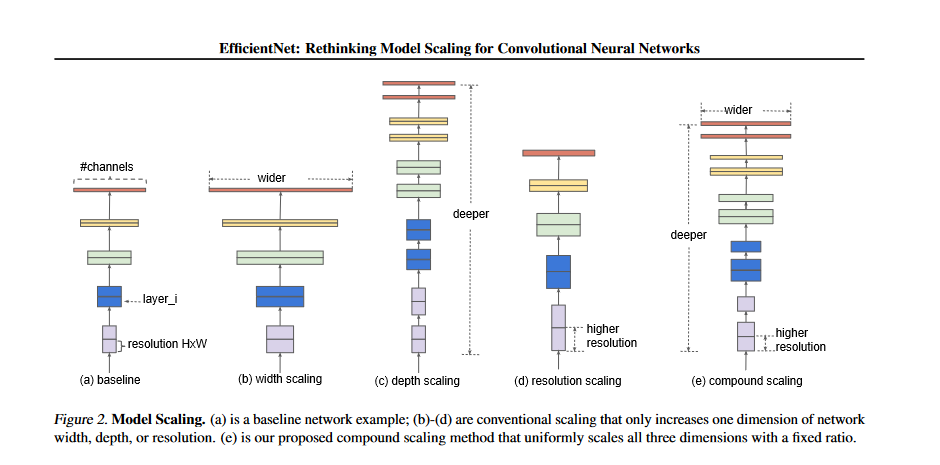
\includegraphics[width=0.8 \textwidth]{plots/efficientnet}
     \caption{Figure 2 from the ConvNeXt paper \cite{efficientnet}. It shows the different approach that deep learning
     model can take to model scaling, compared to their version.}
     \label{fig:efficientnet}

\end{figure}

    EfficientNet was another model improving on the basic building blocks of CNN, in order to improve the efficiency (see \ref{fig:efficientnet}). While it is
    not the best one, this approach has led to further development. Such improvement came in the form of the You Only Look Once (YOLO) object detection
    model, which quickly became a SOTA model. Further improvement have allowed this model to keep its position as one of the best pretrained model publicly available.

    \subsection{Model 4 : Deit \& Transformers \cite{deit} \cite{image16x16}}


        \begin{figure}[h!]

             \centering
             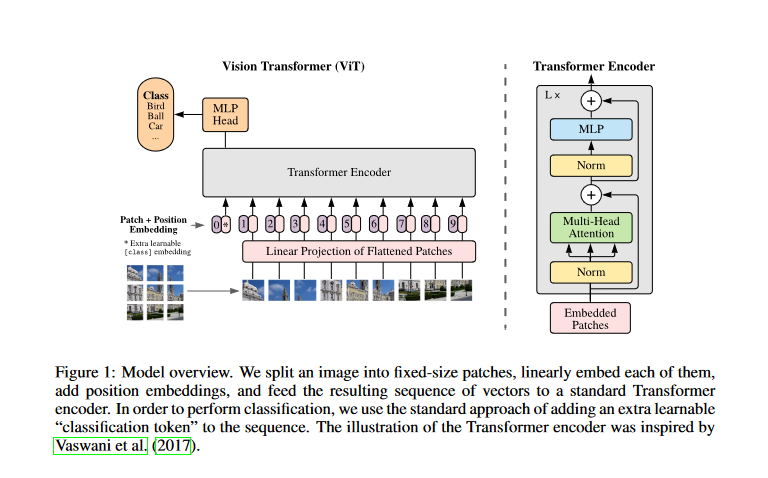
\includegraphics[width=0.8 \textwidth]{plots/transformer}
             \caption{Figure 1 from the An image is worth 16x16 words paper \cite{image16x16}. It shows the general approach of an image transformer.}
             \label{fig:transformer}

        \end{figure}

        Transformers are a new revolution in deep learning. First developped to deal with natural language processing (NLP),
        they were later introduced in image models, successfully improving on CNN's. While CNN still keep a few key
        elements on their side(they usually perform better to extract local information in an image), transformers split the image in blocks,
        treating them as different element of a sequence (see \ref{fig:transformer}). Among other things, this allows them to better extract global feature present in an image.

        Later, the facebook research team improved on this general idea by pre-training the model on a similar, but different task, a now
        common approach when using transformers. This allowed them to achieve a greater accuracy in the ImageNet competiton than previous models.
    

    \section{Training}


    \subsection{Loss function}
        To train a classification model with a multilabel output, we use the Binary Cross Entropy. We therefore treat
        each class as a binary classification problem.

        To account for our dataset imbalance, we will also use weights for the positive example of a class ($P_c$), and weights for the specific classes ($w_c$) such that the loss will be

        \begin{equation}
            L = \frac{1}{N}\sum_{n=0}^N -w_n[p_c y_n log(\sigma(x_n)+(1-y_n) log(1-\sigma(x_n)))]
        \end{equation}

    \subsection{Learning Rate Scheduler}

        We will use a learning rate scheduler to help the model converge faster. We will use a OneCycle learning rate \cite{onecyclelr}, which will
        decrease the learning rate as the training progresses. This will help the model converge faster, and avoid overfitting.

    \subsection{Early stopping}

        Early stopping is a technique used to avoid overfitting. It consists of stopping the training when the validation loss starts to increase. We will
        implement a patience mechanism so that the training will stop only if the validation loss has not improved for a certain number of epochs.
    \subsection{Optimizer}

        Multiple optimizer exists, building on one another . While none is perfect, or definitely better than another, AdamW \footnote{See https://pytorch.org/docs/stable/generated/torch.optim.AdamW.html or \cite{adamw}} is oftenly use as it tends
        to converge rapidly, thus allowing for far smaller training time.

        AdamW is a slightly modified version of the optimizer Adam (which itself is a modified version of AdaGrad and RMSProp), and fixed an error in the L2 regularization from the original implementation.

        AdamW is also chosen as it has demonstrated its abilities to converge easily with the default hyperparameters. This also allows to diminish the needs for finicky hyperparameters tuning.


    \subsection{Experiment Tracking}
        To track our experience, we used Weight\&Biases\footnote{www.wandb.ai} .This tool allows us to track the different hyperparameters,
        the loss, the accuracy, and the model architecture. It also allows us to compare different runs, and to easily reproduce them.
    \subsection{Metrics}
        In any unbalanced dataset, the accuracy won't be enough to determine the performance of a classifier.
        We therefore decided to look into the Area Under the Roc Curve (AUC-ROC) \footnote{https://towardsdatascience.com/understanding-auc-roc-curve-68b2303cc9c5}
        and the F1-score\footnote{https://towardsdatascience.com/the-f1-score-bec2bbc38aa6}.

        While the F1-score does allow to evaluate the performance of our classifier, it requires to first assign a class
        to our model's output. This in turn require to preset a threshold, which, without the results first, will usually be arbitrarily
        chosen to be 0.5.


    \subsection{Classification Head}

        While we use a pretrained model for our feature extraction, leaving us little to change on that side, the classification head is usually a simple fully connected
        layer, allowing us some leniency if we were to want to change it. However, such modification are usually not required for a simple classification model . However , as we switch
        from  classification to object detection, we might want to change this later.

        For now, we might mostly just want to work with the dropout parameter. DropOut is a useful technique to avoid overfitting and increase model
        generalization \footnote{https://towardsdatascience.com/dropout-in-neural-networks-47a162d621d9}

    \subsection{Tips and Tricks}

    \begin{enumerate}
        \item label-smoothing : A common use technique of adding or removing a small value (e.g 0.1) from the label in
        order to smooth out the gradient (e.g $0\xrightarrow{}0.1$ , $1\xrightarrow{}0.9$ )

        \item batch size : Always use a multiple of 2

        \item Clip-Norm : The weight of the model might sometimes grow larger and larger leading to overflow and
        infinite/Nan values! To avoid this, the gradient's norm might be clipped at a maximum value (e.g 1)
        
        \item Timm : The code use the timm library \cite{timm} in order to load a model, allowing
        for an easy use of a multitude of pretrained model.


        \item Input Channels : While models are pretrained to use 3 channels (RGB), we can use a single channel (e.g grayscale). This uses
        only one of the convolution kernel at the first layer of the model, and thus reduce the number of parameters to train. However, it might require more training
        as it will affect the input of all the other layers of the model.

    \end{enumerate}

    \section{Preliminary Results}

        \subsection{Reproducing CheXpert baseline}

            While we do not have access to the hidden test set from CheXpert, we still have access to their validation dataset. However,
            as can be seen in \ref{fig:histogram_chexpert_valid}, three classes are not available in the validation dataset. We will therefore have to
            limit our comparison to the classes present in the validation dataset , and to keep in mind our results will
            most likely be higher than they would be on the test set. However, to keep things simple, we will not proceed to model ensembling as this
            will simply put a high computational cost for a simple verification step.


    Doing so , we can see our results in the figure\ref{fig:CheXpert_baseline}. While our results are slightly lower than
    the values reported by the CheXpert team, we however achieve close enough value to be confident in our implementation.
    However, only 5 classes were reported in the paper, and we have 11 classes. We will therefore have to compare our results with other sources.

    If you paid attention up to this point, you will also have notice that CheXpert had 14 classes, and not exactly the same as we have!
    This is due to a talk with our radiologist, where they identified some classes as being too similar to be useful, and we thus removed them. They also pointed they would like to have
    more general labels, such as \"Air\", \"Liquid\" and \"Opacity\", which regroups other classes (see \ref{fig:pathologies_hierarchy}). This is something we will keep in mind for the future.



        \begin{figure}[h!]

             \centering
             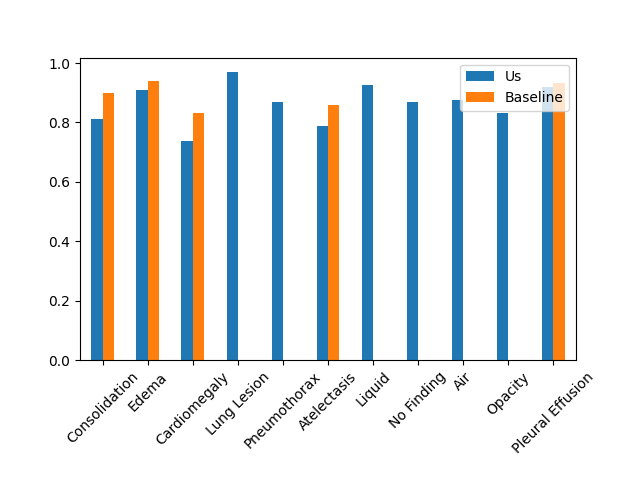
\includegraphics[width=0.8 \textwidth]{plots/chexpert_baseline_blue+comparison}
             \caption{Attempt at reproducing the chexpert baseline. Results for the baseline are taken from \cite{chexpert}}
             \label{fig:CheXpert_baseline}

        \end{figure}

        To obtain these results, we used the following hyperparameters :

        \begin{itemize}
            \item backbone : convnext\_small
            \item batch size : 64
            \item learning rate : 1e-3
            \item weight decay : 1e-2
            \item dropout : 0.2
            \item num\_samples\_per\_epoch : 50\_000
            \item optimizer : AdamW
            \item scheduler : OneCycle
            \item patience : 5
            \item label smoothing : 0
            \item clip norm : 1
            \item epoch : 50
            \item channel : 1
            \item augment prob 1 1 0.5 0 0 %TODO : ADD a description of this in data augment
        \end{itemize}

        The positive weights were calculated using the following formula : $pos\_weight = \frac{N_{neg}}{N_{pos}}$ where $N_{neg}$ is the number of negative samples, and $N_{pos}$ is the number of positive samples for a given class. Their value range
        in between 1 and 95. The values are reported in the table \ref{table:pos_weight_chexpert}. I suspect that high values might scramble the loss for the batches containing the rare positive samples of that class. We might later want to cap
        the maximum possible value of the positive weight to avoid this.



        \begin{table}[h!]
            \centering
            \begin{tabular}{@{}lllll@{}}
            \toprule
            Classes          & & & & Weights \\ \midrule
            Opacity          & & & & 1.97    \\
            Air              & & & & 16.76   \\
            Liquid           & & & & 1.16    \\
            Cardiomegaly     & & & & 12.15   \\
            Pleural Other    & & & & 94.76   \\
            Pleural Effusion & & & & 3.07    \\
            Pneumothorax     & & & & 21.06   \\
            Lung Opacity     & & & & 1.68    \\
            Atelectasis      & & & & 9.66    \\
            Lung Lesion      & & & & 27.71   \\
            Pneumonia        & & & & 50.26   \\
            Consolidation    & & & & 33.28   \\
            Edema            & & & & 6.11    \\
            Fracture         & & & & 22.77   \\
            No Finding       & & & & 6.58    \\ \bottomrule
            \end{tabular}
            \caption{Positive weights used for the loss , from the CheXpert dataset}
            \label{table:pos_weight_chexpert}
        \end{table}

        For CheXpert, all the training examples were sampled with equal weights.


        \subsection{Reproducing the CheXpert competition's results}

            The CheXpert dataset was released as part of a competition, where the goal was to achieve the best possible performance on the hidden test set. The competition was won by a team from Stanford, who achieved a score of 0.91 on the hidden test set. The results of the competition are reported in the table \ref{table:chexpert_competition_results}.
            The metric used was the ROC-AUC. We will therefore use the same metric to compare our results with theirs. However , we also implemented the
            F1-score (the harmonic mean of the precision and recall), which will make it easier to compare with the radiologist's performance
            in order to convince them to use our model.


            \subsubsection{DeepAUC \cite{DeepAUC}}

                Attempting to reproduce the results of DeepAUC \cite{DeepAUC} proved not to be possible. The snippet of code , provided by the author,
                did not reproduce the results as expected. No pretrained model was also given. Attempt to use their loss function with our dataset also proved
                to be unsuccessful. We therefore decided to not include their results in our comparison, and to not pursue this avenue.

            \subsubsection{Hierarchical Learning \cite{hierarchical}}

                    The hierarchical learning method \cite{hierarchical} is a method that uses a hierarchy in between the different classes
                    to more accurately predict them. Thansk to bayesian probabilities, we know that

                    \begin{equation}
                        P(A|B) = \frac{P(A \cap B)}{P(B)} = \frac{P(B|A) P(A)}{P(B)}
                    \end{equation}

                    If we use the parent class as B, with the child class as A, we can therefore redefine
                    the probability of the child class such that

                    \begin{equation}
                        P(Child|parent) = \frac{P(Child \cap parent)}{P(parent)} \approx P(parent|Child) P(Child)
                    \end{equation}

                    We could use P(Parent) as the prior probability of the parent class, as defined by the preponderance in the dataset. However, as I base myself of
                    \cite{hierarchical}, I observe they did no such thing and I decided to not do it either. While this mean the probability given by the model might be based off an approximation,
                    it also avoids having an additional bias in the model originating from the specific distribution of the training set. Further thought might however be given to this in order to evaluate the potential benefit of it.

                    Since the classes we are interested in slightly differ from the ones used in \cite{hierarchical},
                    we will have to adapt the hierarchy. The hierarchy used in \cite{hierarchical} is reported in the figure \ref{fig:hierarchical_learning_hierarchy}. We will use the same hierarchy, but with our classes instead of theirs.
                    We will then compare with and without to see if the results improve.



            \subsubsection{JFHealthcare - Probabilistic-CAM \cite{jfhealthcare}}

            \begin{figure}[h!]

                 \centering
                 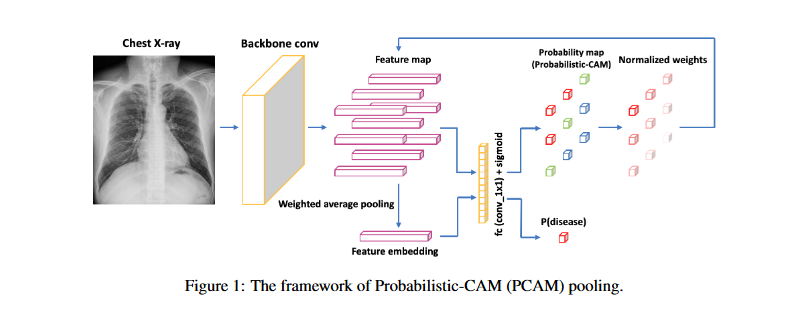
\includegraphics[width=0.8 \textwidth]{plots/jfhealthcare}
                 \caption{The figure 1 from \cite{jfhealthcare}}
                 \label{fig:jfhealthcare_probabilistic_cam}

            \end{figure}

            The JFHealthcare team \cite{jfhealthcare} used a probabilistic-CAM method to obtain their results.
            The method is based on the idea that the model should be able to predict the probability of a class being
            present in the image. The method is described in the figure \ref{fig:jfhealthcare_probabilistic_cam}.

            They first start by proceeding as usual, applyng a feature extraction backbone, followed by a 1x1 convolutionnal layer.
            They then apply a sigmoid activation function to the output of the fully connected layer, in order to obtain a probability between 0 and 1.

            These classes probability are then used as the probability of a disease being present in each of the feature maps. The feature maps are then
            weighted according to these probabilities using a weighted average pooling. This is then followed by a fully connected layer (with a sigmoid activation), which is used to output
            the final prediction.


            This adds two benefits . The first one is to enable a form of self-attention within the model which they have shown increase the accuracy of the model.
            But further than that, it also allows for a better understanding of the model's decision. Indeed, the weighted class activation maps offer a more accurate way to visualize the model's decision and potential object location
            within the image. This is especially useful for the radiologist, who might want to understand why the model made a certain decision.


        \subsection{Results on the CIUSSS dataset}


            Following the results obtained earlier on CheXpert, we then tried applying some of the same technique, but this time using a validation dataset from the CIUSSS data.
            For the training data, we tried to supplement the CIUSSS dataset with the CheXpert dataset, in order to increase the size of the dataset and improve the model's performance.



    \section{Analysis of the results}



    \section{Improvements and attempts}

    \subsection{Moving Average Labels}


    \section{Problem observed}

    A multitude of problems slowed down the development of the model. We will try to cover the most
    important ones here, and the lesson learned from them.


    \subsection{Normalizing the data}

        While the data was at first simply normalize by the mean and standard deviation of the ImageNet dataset.
        However, we realized this was not enough . This easily led to unstability in the training process, and we had to further
        normalize the input. The first attempt at this was with a min max normalization to rescale between 0 and 1, before applying the ImageNet's normalization
        .While this solved the issue, we did try to further improve the normalization by using the CLAHE algorithm. This algorithm is used to improve the contrast of the image, and is often used in medical imaging.

    \subsection{Verifying the data}
            The data was not as cleaned as we would have liked. While the CheXpert validation dataset was validated by a team of three radiologist, our data
            was simply annotated by a single radiologist's report, from which the labels were then automatically derived. This lead to a quite important source of error as radiologist's performance
            is estimated to be between 0.4 and 0.6 \cite{radiologist_performance}. This is a quite important source of error, which is compounded
            by the fact that the radiologist's report often contained many uncertainties that we had
            to quantify with an automated labeler. The problem's come that no radiologist was available to verify the work of the labeler, and we had to rely on our interpretation of
            the report to evaluate the performance of the rule-based labeler we developped.

            While it usually would simply be solved by manually annotating a few examples and compare the results accrosss the manually labeled dataset
            and the automatically labeled one, this was not possible in our case. Indeed, the nature of our medical dataset required an expert eye to verify the data,
            and even then, radiologists often disagree on the label of a given image. This is why when working on medical data, it is important to have a team of specialist available to support the project.


    \subsection{Drivers \& CUDA}

        Many times did we had issues with our drivers. This happened because we were updating the packages as we were developping the project, and because we were working on parallel on more than one project
        on the same machine. To rectify and avoid this, a simple solution is to use a virtual environment, which will allow us to have a clean environment for each project, and to avoid any conflict. Docker
        is a good solution to provide such virtual environment.

    \subsection{Multi-GPU training}

        To train on multiple GPU, I first used the DataParallel module from PyTorch. However, this module is deprecated, and I therefore chose to switch to the DistributedDataParallel module. This module is more efficient, but it is also more complicated to use.
        Just as to prove this point, it often break down, seemingly at random, and I had to restart the training process.

        While in and of itself it would only be annoying, the real problem is that the training would not simply stop, but would not converge, leading to
        wrong conclusion when trying to compare the results of the different models. It seems like the problem might arise from the synchronization of the
        gradient between the batches on each GPU. You see, compared to data parallel, the distributed data parallel instead of splitting the model between the GPUs, it splits the data between the GPUs.
        This means that the gradient are computed on each GPU, and then synchronized between the GPUs.

        This is a problem that I have not been able to solve, and I have not been able to find any solution to it online. I have therefore decided to switch back to the DataParallel module, which is less efficient, but at least it works.


    \subsection{Data augmentation}


        At first, I tried to implement a few technique of data augmentation of my own, as the torchvision library does not provide a lot of data augmentation technique.
        However, I quickly realized that the data augmentation technique I implemented were not as good as I wanted, being both not optimized enough and containing errors I would catch from time to time.

        Later, I found the Albumentations library \cite{albumentations}, which is a library that provides a lot of data augmentation technique, and is very easy to use. I therefore decided to switch to this library, and it has proven to be a very good choice.
        It allowed me to quickly and easily test a few different data augmentations without worrying about potential errors in my implementation.

        However, it is not idiot-proof either. As I was working on the project, I later found a bug where my image input of format (C,H,W) was not being converted to (H,W,C) by the library, as it required, but was still processed, leading to disastrous images.

        To avoid this step, a jupyter notebook was then used to verify the output of our dataloader at different step in order to verify the integrity of the image
        throughout its pre-processing.

    \subsection{Unitary Tests}

            Based on the experience described above, I also decided to implement unitary testing in order to limit the errors
            that could be introduced in the code. The master branch of the git repository was also linked to these unitary tets such that
            any pull requests would first have to pass the tests before being merged into the branch. This is especially useful when working with a group,
            but even when working alone it is a good way to ensure that the code is working as intended and catch unintentional errors.


    \subsection{Unstability during training}

    \subsubsection{Automatic Mixed Precision (AMP)}

            To solve this problem, I tried to implement the automatic mixed precision (AMP) technique \cite{automatic_mixed_precision}. This technique is a way to train a model in a lower precision, while still using a higher precision for the gradient computation.
            This is especially useful when training on a GPU, as it allows to reduce the memory usage, and therefore to train on larger batch size.

            However, this technique is not without its problems. Indeed, it is not always easy to implement, and it is not always compatible with all the libraries used.
            While this technique improved the training time vastly, it did lead to some unstability, with the gradient sometimes underflowing and becoming NaN.

            This is a problem that I have mostly solved by normalizing further the input vector but some underflowing might still occur. In these case, the training need to be done
            again as the model will be corrupted (Nan values in the weights).


    \subsubsection{Gradient's clipping}

        While we already experienced some unstability before, we mostly tried to solve it by normalizing the input.
        However, we still had some issues with the training process. To avoid overflowing gradients, we tried to use the gradient clipping technique \cite{gradient_clipping}.
        This technique is a way to limit the gradient to a certain value, in order to avoid them from exploding.

        By default, we set the maximum gradient norm to 1, but we also tried to set it to 2, and to 5. However, we found that the best results were obtained with a maximum gradient norm of 1.
        This also serves as a way of regularizing the model, as it forces the gradient to be small, and therefore forces the model to learn slowly.


    \newpage
    % REFERENCES
    {
    \small

    \printbibliography
    }
\end{document}